%%
%% This is file `example-1.tex',
%% generated with the docstrip utility.
%%
%% The original source files were:
%%
%% drexel-thesis.dtx  (with options: `example-part')
%% 
%% This is a generated file.
%% 
%% Copyright (C) 2010 W. Trevor King
%% 
%% This file may be distributed and/or modified under the conditions of
%% the LaTeX Project Public License, either version 1.3 of this license
%% or (at your option) any later version.  The latest version of this
%% license is in:
%% 
%%    http://www.latex-project.org/lppl.txt
%% 
%% and version 1.3 or later is part of all distributions of LaTeX version
%% 2003/06/01 or later.
%% 

\chapter{Methods}

\section{Neuron model}
To study traveling waves in small columnar ensembles (SCE) of neurons we created a MATLAB simulation of our model based on \citet{izhikevich2003}.
We model the firing dynamics of each neuron using the Izhikevich model \citep{izhikevich2003} that consists of a two-dimensional model of two coupled differential equations given by:
\begin{align}
 \begin{split}
  v^\prime &= 0.04v^2+5v+140-u+I \label{eq:neuron_v} \\
  u^\prime &= a(bv-u)
 \end{split}
\end{align}
where $v$ is the membrane potential of the neuron and $u$ is a membrane recovery variable, with a spike threshold and an auxilliary after-spike resetting of parameters by:
\begin{align}
  \text{if } &v>30: v\leftarrow c, u\leftarrow u+d
\end{align}
and I is the sum of all incoming currents to the neuron, explained in detail below. 

Equation \ref{eq:neuron_v} has four parameters (a,b,c,d) that with specific values can model a wide range of neuronal spiking behavior \citep{izhikevich2003}. 
The parameters used here (see Table \ref{tab:izzy_params}) are based on the original model with modification of the $c$ parameter for excitatory neurons and define a random population of neurons where $U(s,t)$ represent a number drawn from a uniform random distribution between s and t. 
\begin{table}[!htb]
 \caption{Izhikevich model parameters}
 \label{tab:izzy_params}
 \centering
 \begin{tabular}{lcr}
  \textbf{Parameter} & \textbf{Excitatory} & \textbf{Inhibitory} \\
  \hline
  a & 0.02 & 0.02+$\mathcal{U}$(0,0.08) \\
  b & 0.2 & 0.25-$\mathcal{U}(0,0.05)$\\
  c & -65+$\mathcal{U}(0,10)^2$ & -65 \\
  d & 8-$\mathcal{U}(0,6)$& 2 \\
 \end{tabular}
\end{table}
For solving equation \ref{eq:neuron_v} numerically we use the modified Euler method from \citet{izhikevich2003} with a time step of $0.2 ms$ except were noted. 

The current I in equation \ref{eq:neuron_v} includes the sum of all incoming stimuli into neuron $i$ from other neurons $I_i$ and external stimuli $I_{i,e}$ applied to the system. 
The neuron-neuron incoming current $I_i$ into neuron $i$ is given by:
\begin{align}
 I_i(t) &= \sum_{j\ne i} \sum_{t^\prime_j} S_{ij}  \Theta(t-t^\prime_j-\tau_{ij})e^{-(\frac{t-t^\prime_j-\tau_{ij}}{\sigma_s})^2}
\end{align}

where $t'_j$ are the firing times of neuron $j$, $\Theta$ is the Heaviside step function, and the exponential factor models an exponentially decaying synapse response with a time constant of $\sigma_s = 4 ms$. 
The $S_{ij}$ represent the connection strengths between presynaptic neuron $j$ and postsynaptic neuron $i$ given by
\begin{align}
 \begin{split}
  S_{ij}^{excitatory} &= K \times \mathcal{U}\{0,0.5 \} \\
  S_{ij}^{inhibitory} &= K \times \mathcal{U}\{-1,0 \}  \\
 \end{split}
\end{align}
where $K$ is a parameter that modulates the strength of connections, with $K=1$ corresponding to the original model in \citet{izhikevich2003}. 

The distribution of Izhikevich model parameters results in variations between our excitatory and inhibitory neurons, as well as variation in the neurons within those classes.
We examine the inter-spike interval (ISI) and its inverse, the spike frequency, for the excitatory and inhibitory neurons in our model.
We generate 1600 excitatory or inhibitory neurons and drive them with a constant stimulus, measuring the resulting ISI/spike rate as shown in Figure \ref{fig:ISIstatistics}.
The inhibitory neurons spike at a lower input level and the spike rate rises more quickly with stronger input.
Due to the stochastic variation in the 'b' parameter for inhibitory neurons, different inhibitory neurons can have a different minimum firing threshold.
Starting at an input magnitude of $4\ mV$, at which all the inhibitory neurons fire, the spike rate of the inhibitory neurons increase linearly with the input magnitude with a slope of 13.
The excitatory neurons all have a common firing threshold.
The spike rate of the excitatory neurons increases linearly with the input magnitude, and the slope of the linear fit is 3.
\begin{figure}[!htb]
  \subfloat[][]{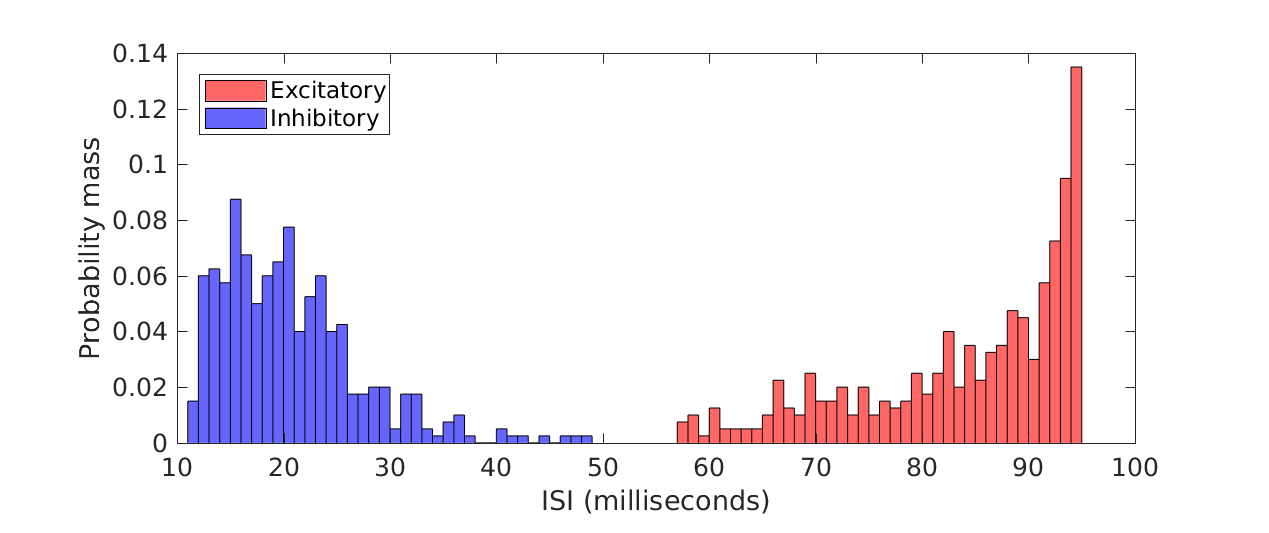
\includegraphics[width=0.75\textwidth]{fig/ISIDistribution} } 
  \subfloat[][]{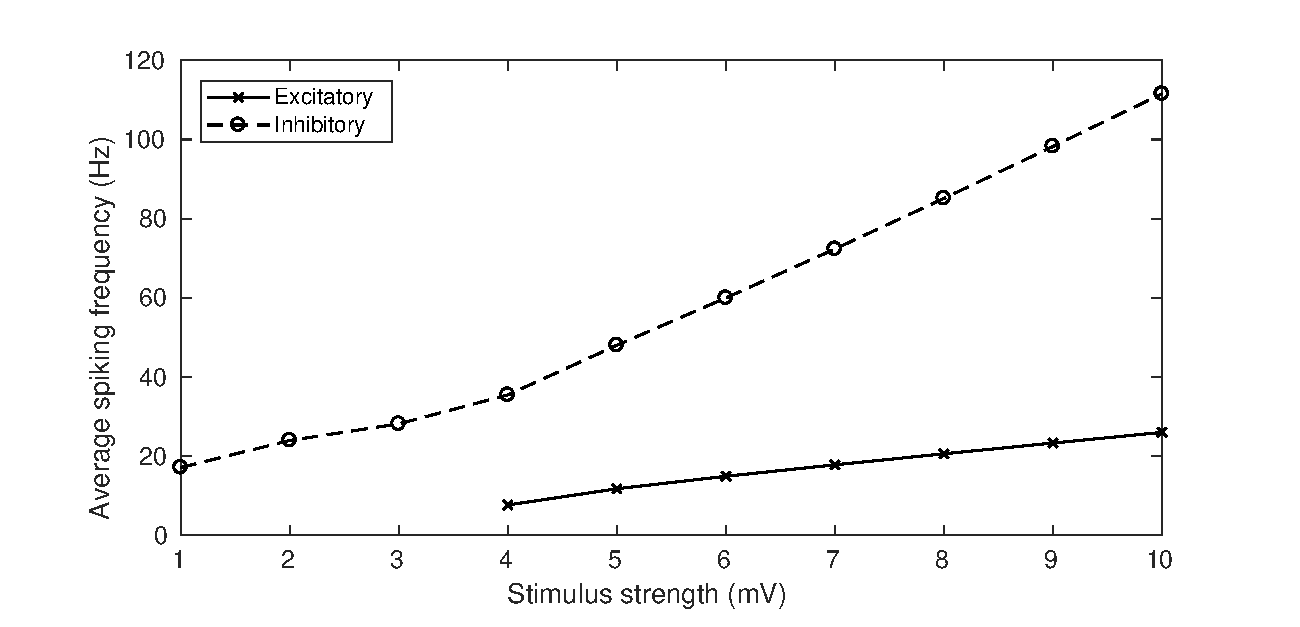
\includegraphics[width=0.75\textwidth]{fig/AvgSpikeFrequency} }
  \caption{a) The distribution of inter-spike intervals for our excitatory and inhibitory neurons with a constant $5\ mV$ stimulus.  
      b) The spike frequency of the excitatory and inhibitory neurons increases as the constant stimulus becomes stronger.}
  \label{fig:ISIstatistics}
\end{figure}
\FloatBarrier

\section{Neuron stimulus}
To drive the firing dynamics and create traveling waves we provide stimulation to the systems by using two different and separate external stimulus currents, $I_{i,e}$. 
One of them is a uniform background stimulus applied to each neuron $k$ that depends on whether the neuron is excitatory or inhibitory.
The stimulus values are drawn from a random distribution every $1 ms$ according to:
\begin{align}\label{eq:randomstim}
 \begin{split}
  I_k^{excitatory} &= M \times \mathcal{U}\{0,1 \} \\
  I_k^{inhibitory} &= \frac{2}{5} M \times \mathcal{U}\{0,1 \}
 \end{split}
\end{align}
where $M$ is a parameter that tunes the overall strength of the stimulus, with $M=5$ corresponding to the original model in \citep{izhikevich2003}. 
This stimulus has the effect of creating waves that originate from any point along an SCE and one of the uses is to study interactions between multiple waves in section \ref{sub:wave_initiation}.

The other external stimulus $I_{i,e}$ is a short constant input of current applied to all of the neurons in one area of a system. 
The duration of the stimulus is $20 ms$ with a strength of $5 mV$. 
This stimulus has the effect of creating a single wave with a well-defined starting location and time.
One of the uses of this stimulus is to measure the speed of the traveling wave in section \ref{sub:propagation_speed}.

\section{Neuron connectivity}
We first construct these assemblies by placing neurons at the vertices of a cubic lattice with coordinates X, Y and Z. 
Each neuron is  randomly chosen to be  either excitatory (E) or inhibitory (I), with the fraction of excitatory neurons indicated as $P_{exc}$.
After placing, we connect two neurons based on their relative distance according to a connection probability that favors local connectivity given by  \citep{maass2002}: 
\begin{align}\label{eq:connectivity}
 P_{a,b} &= C e^{-(D(a,b)/\lambda)^2}
\end{align}
where $D(a,b)$ is the Euclidean distance between neuron a and b, $\lambda$ is the characteristic length of the local connectivity neighborhood, and $C$ is the peak probability of connection .
In \citet{Levy2012} the authors showed that the synaptic connections in the mouse auditory cortex follow this connection probability.
Multiple connections from the same presynaptic neuron to the same postsynaptic neuron, as well as self-connections, are prohibited.
Two neurons may be recurrently connected, however. 

\section{Model summary}
We summarize our model parameters in Table \ref{tab:all_params}. 
\begin{table}[!htb]
 \caption{Model Summary}
 \label{tab:all_params}
 \centering
 \begin{tabular}{c}
  \textbf{Model} \\
  \hline \\
 \end{tabular} \\
 \begin{tabular}{ll}
  Population & Excitatory, inhibitory \\
  Topology & Quasi 1-D minicolumn, quasi 2-D sheet, ``2.5D'' forest of minicolumns \\
  Connectivity & Stochastic, $P_{connect}$ exponentially decays with distance between neurons \\
  Neuron model & Izhikevich model with distribution of neuron parameters \\
  Synapse response & Exponential synaptic response with randomized peak connection strength  \\
  Spike propagation & Delay proportional to distance, Fixed propagation time \\
  Input & Random input to all neurons, Fixed stimulus to neurons at the bottom of the SCE \\
 \end{tabular}
\end{table}


\endinput
%%
%% End of file `example-1.tex'.
